\chapter{Results \label{ch:results}}
The ID lines are analysed by the program \verb|att_eval.py| introduced in section \ref{sec:meth:data_interpretation}. The

\section{Calibration \label{sec:res:calibration}}
The unfiltered measurements of the magnetometer are presented in fig. \ref{fig:res:raw_cali}. Three bigger spots can be seen, which do not lay on the sphere, as well as some single measurement points distributed throughout the figure. The first step is to eliminate these statistical outliers as explained below.

\begin{figure}[H]
    \centering
    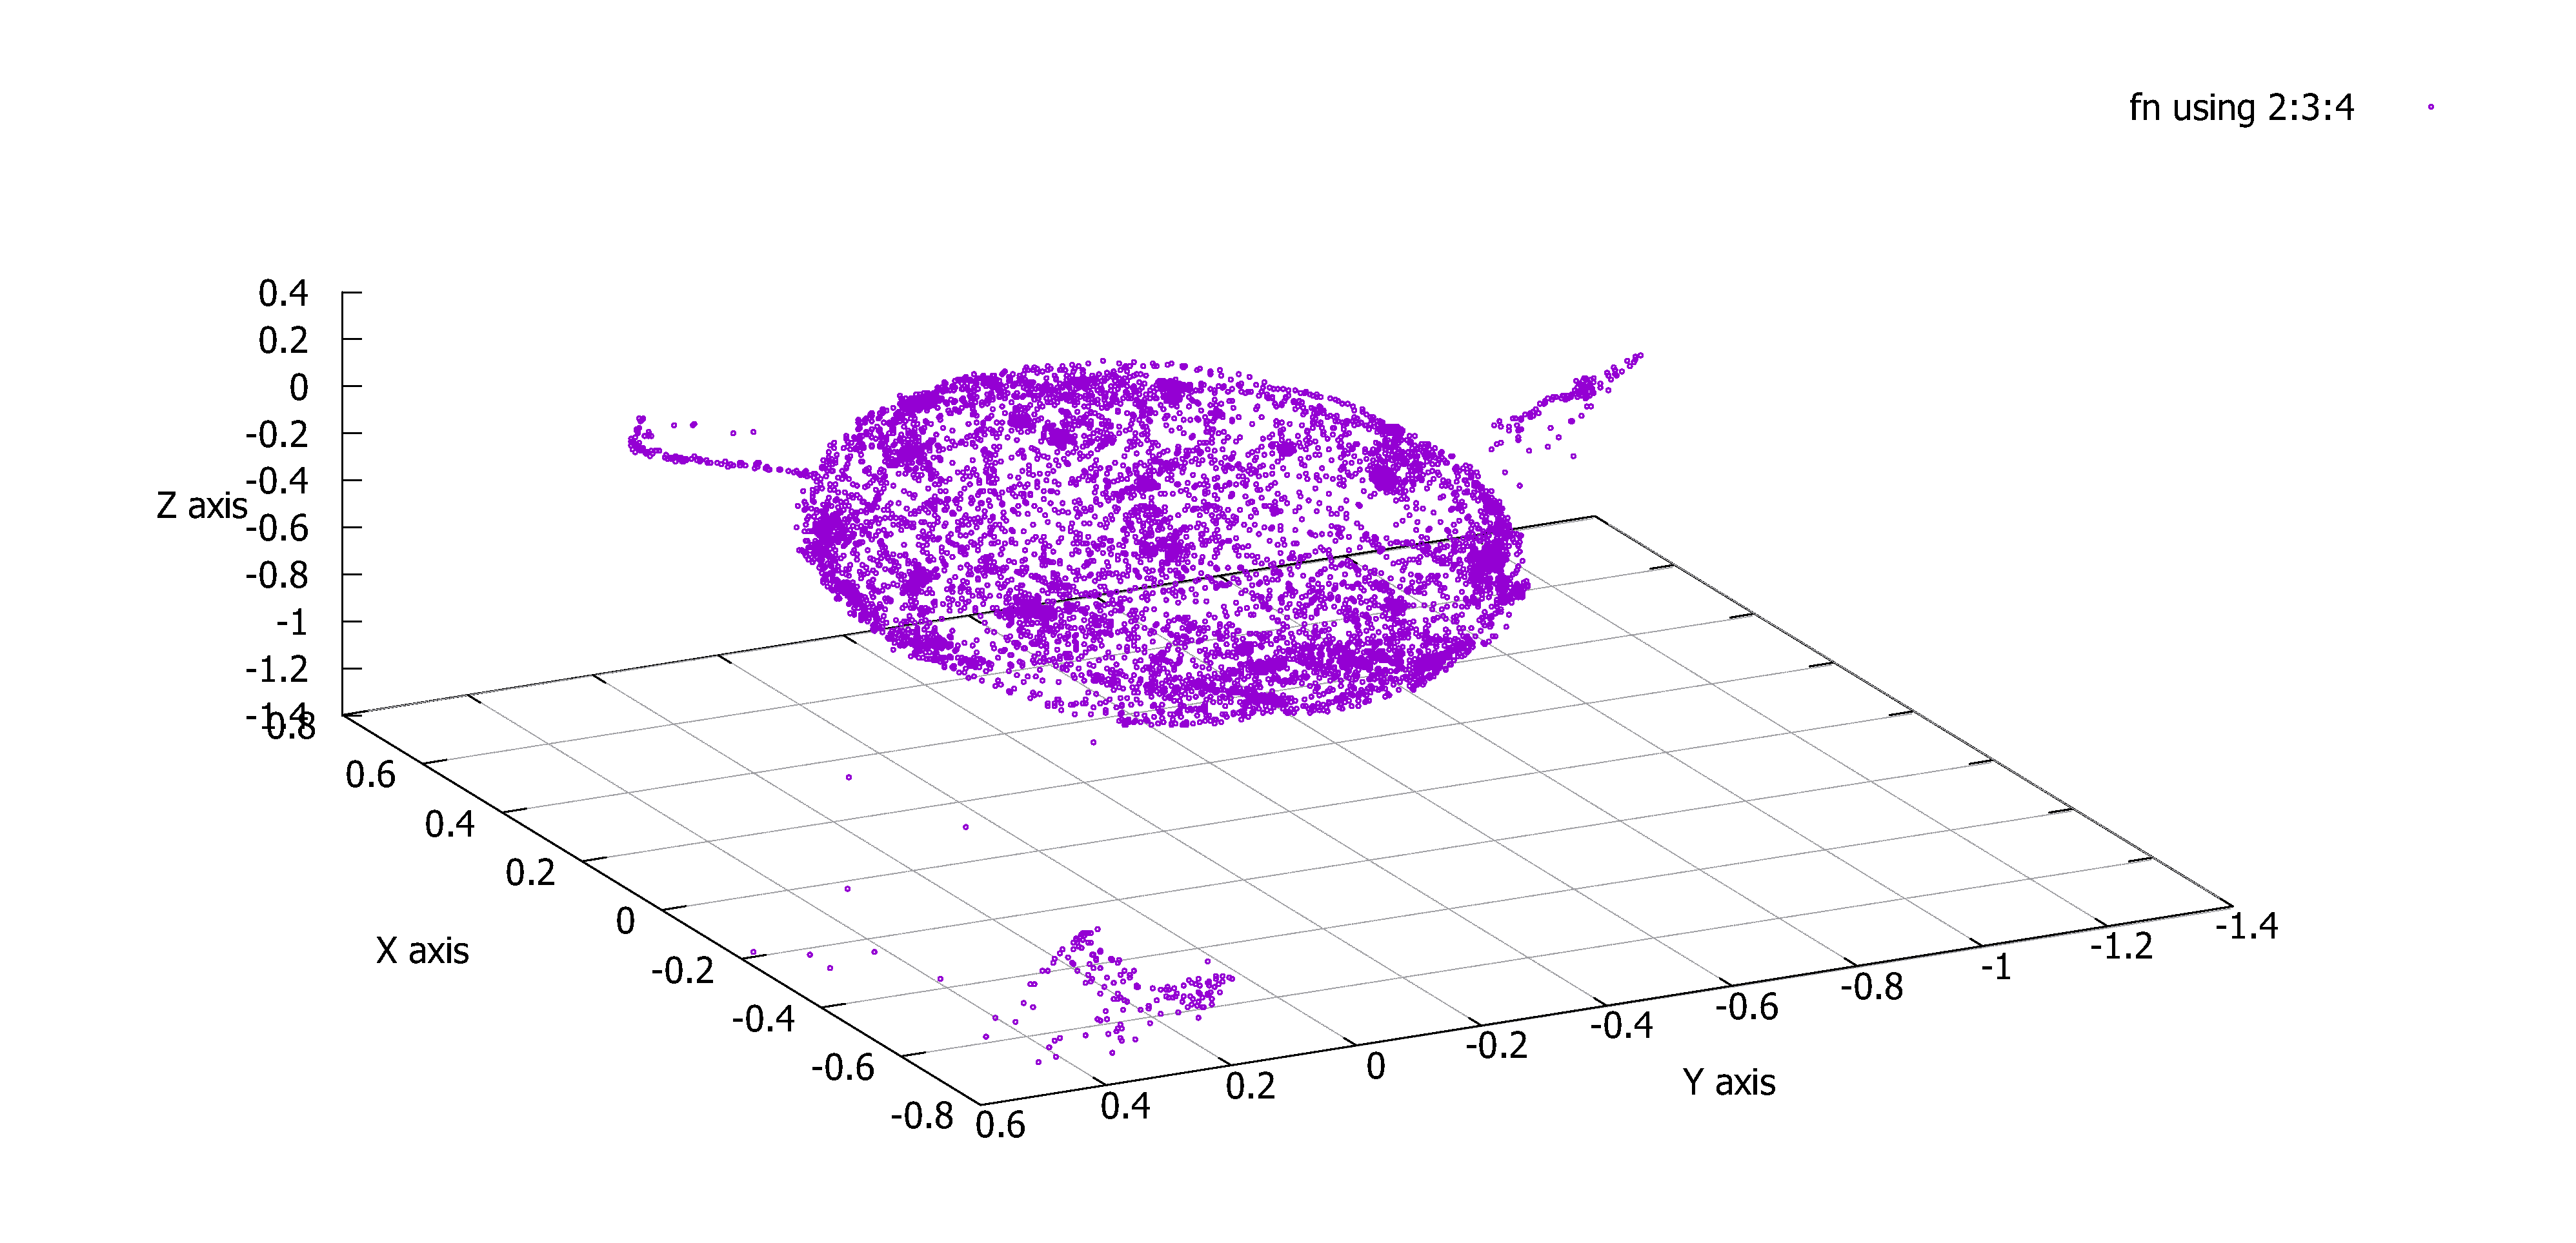
\includegraphics[width=0.8\linewidth]{images/04_results/raw_sphere_2025-04-11.pdf}
    \caption{Components of the magnetometer of the calibration measurement on 11 April 2025 plotted in 3D-Space to form a distorted sphere.}
    \label{fig:res:raw_cali}
\end{figure}

In fig. \ref{fig:res:raw_cali_vectors} the three components of the magnetometer and accelerometer are plotted against their timestamp. This time is incorrect, as the \ac{FPGA} simply continues counting up from the last time it was connected to the internet. That the timestamp is incorrect does not matter for the sensor calibration, as only the time order of the vectors is relevant, rather than their absolute time. In the figure there can be made a clear distinction between three time intervals. The first interval is from the beginning of the measurement until 9:55. This is the time it took to leave the lab, take the elevator to the basement and go to the car park. A lot of vibration can be seen in the accelerometer and stray magnetic fields measured by the magnetometer.\\
The second phase is from 9:55 to around 10:21. After this time is when the random tumble begins. In phase II it can be seen how the magnetometer and accelerometer react to laying the device housing down in different orientations. When rotating the sensors, small shocks can be seen, such as at 10:06. These shocks are a different type of outlier in fig. \ref{fig:res:raw_cali}. The magnitude of the field randomly decreases significantly leading to measurement points near the centre of the sphere.

\begin{figure}[H]
    \centering
    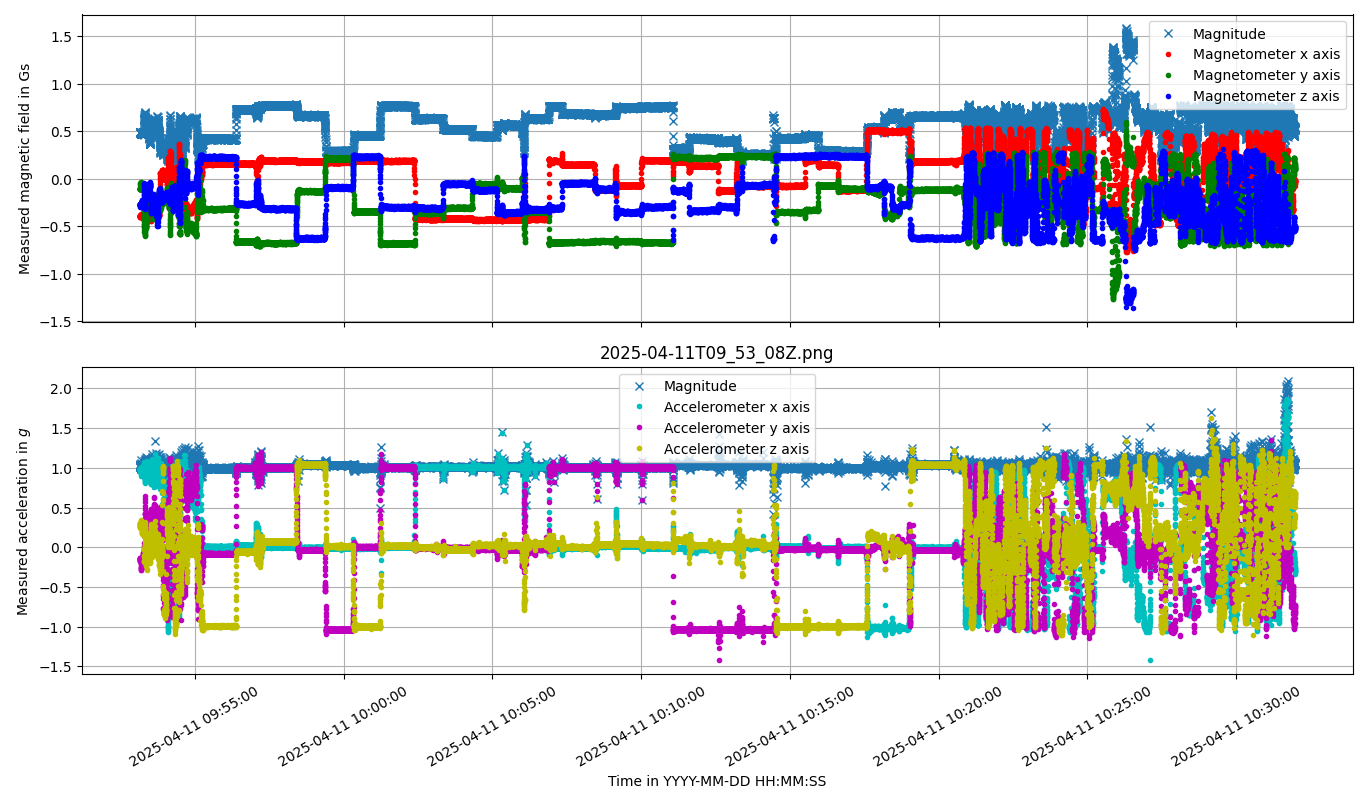
\includegraphics[width=\linewidth]{images/04_results/raw_vectors-2025-04-11.png}
    \caption[Components of the magnetometer and accelerometer plotted against time.]{Components of the magnetometer and accelerometer plotted against time. Shown with blue crosses is the sum of the squares of the components, i.e. the length of the measured vector.}
    \label{fig:res:raw_cali_vectors}
\end{figure}

There is one very important thing we can learn from figure \ref{fig:res:raw_cali_vectors}. The uncalibrated magnetometer measurements are shockingly unreliable. Firstly it can be seen that no particularly sudden or strong accelerations are experienced during the random tumble. However for some reason the magnetometers measured field goes up to about 1.5\,Gs which is around 6 times the field in Kiel (see sec. \ref{sec:da:vector_fields}). Secondly the measured field's magnitude should be roughly constant throughout the whole time of phases II and III when the device is brought outside, away from any hard iron sources. However looking at 10:00 it is blatantly obvious that this is not the case at all, as the offsets and scale factors are different fro each axis not yet determined.\\
We will perform three approximations of these calibration parameters. The first only taking phase II into account, the second only taking phase III into account and the third approximation with both phases. In fig. \ref{fig:res:raw_calibration_three_phases} the components of the magnetometer are shown in all three dimensions to illustrate the different measurement methods of placing the magnetometer in a single position for a longer duration of time (fig. \ref{fig:res:raw_calibration_three_phase_II}) and the random tumble (fig. \ref{fig:res:raw_calibration_three_phase_III}). The time intervals around 10:26 and 10:32 where magnetometer and accelerometer magnitude are significantly higher have been cut, to improve the accuracy of the final parameters.

\begin{figure}[h]
\begin{subfigure}[t]{.33\textwidth}
  \centering
  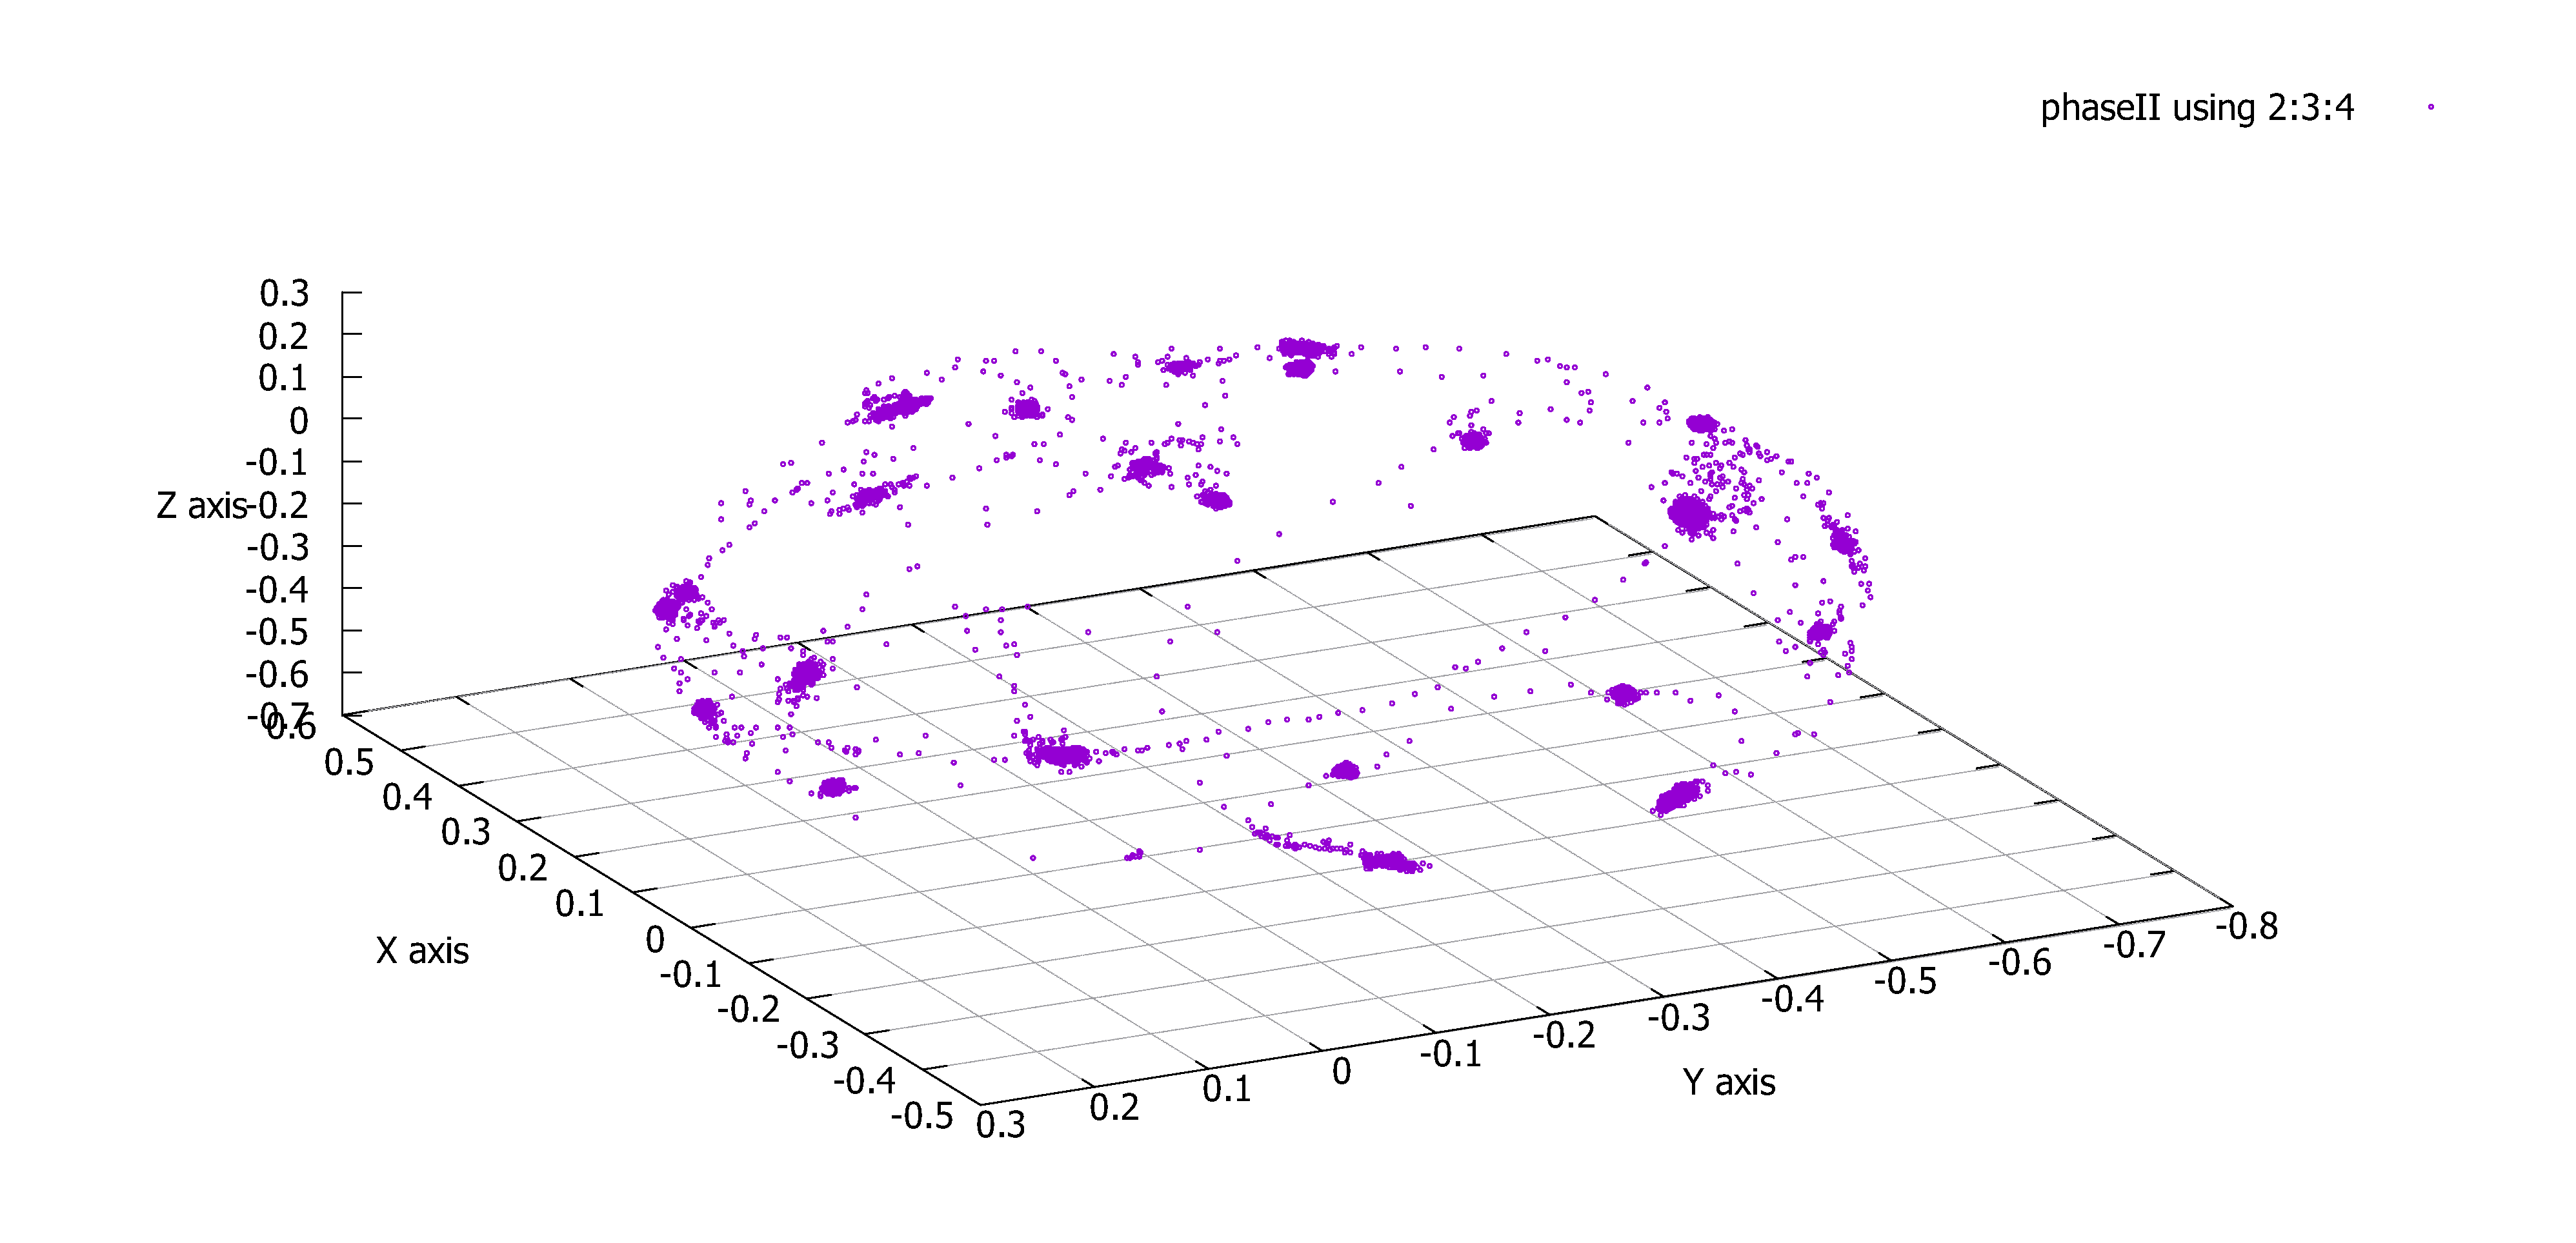
\includegraphics[width=.8\linewidth]{images/04_results/raw_sphere_calibration_phase_II.pdf}
  \caption{Phase II, multiple orientations.}
  \label{fig:res:raw_calibration_three_phase_II}
\end{subfigure}%
\begin{subfigure}[t]{.33\textwidth}
  \centering
  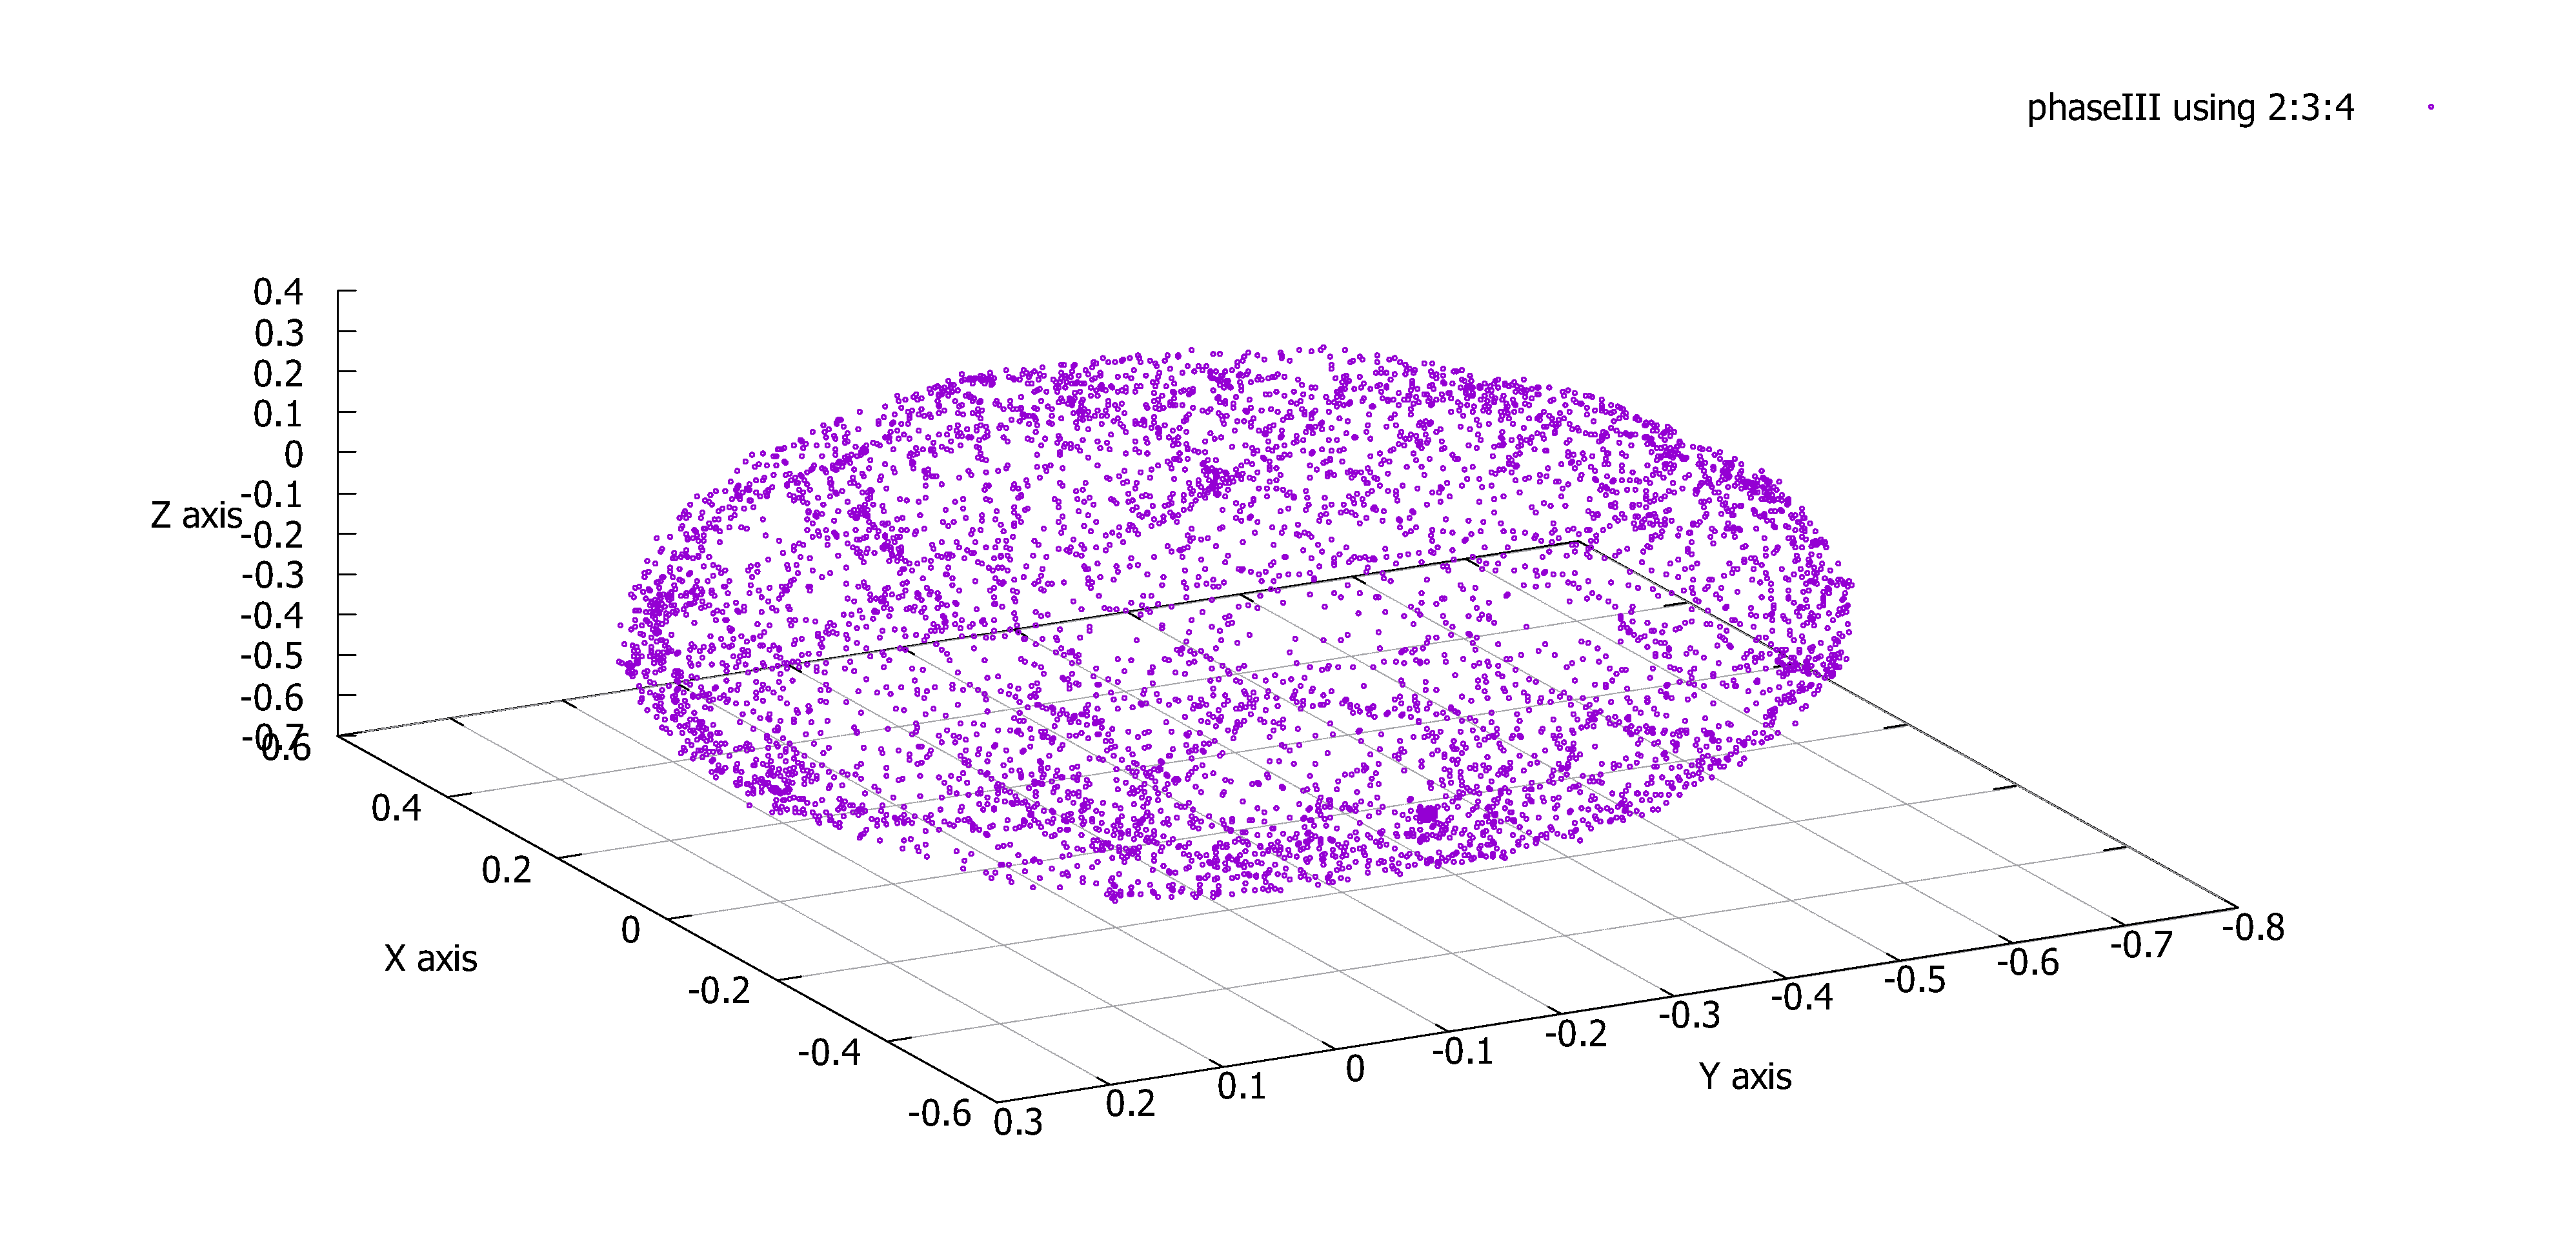
\includegraphics[width=.8\linewidth]{images/04_results/raw_sphere_calibration_phase_III.pdf}
  \caption{Phase III, random tumble.}
  \label{fig:res:raw_calibration_three_phase_III}
\end{subfigure}
\begin{subfigure}[t]{.33\textwidth}
  \centering
  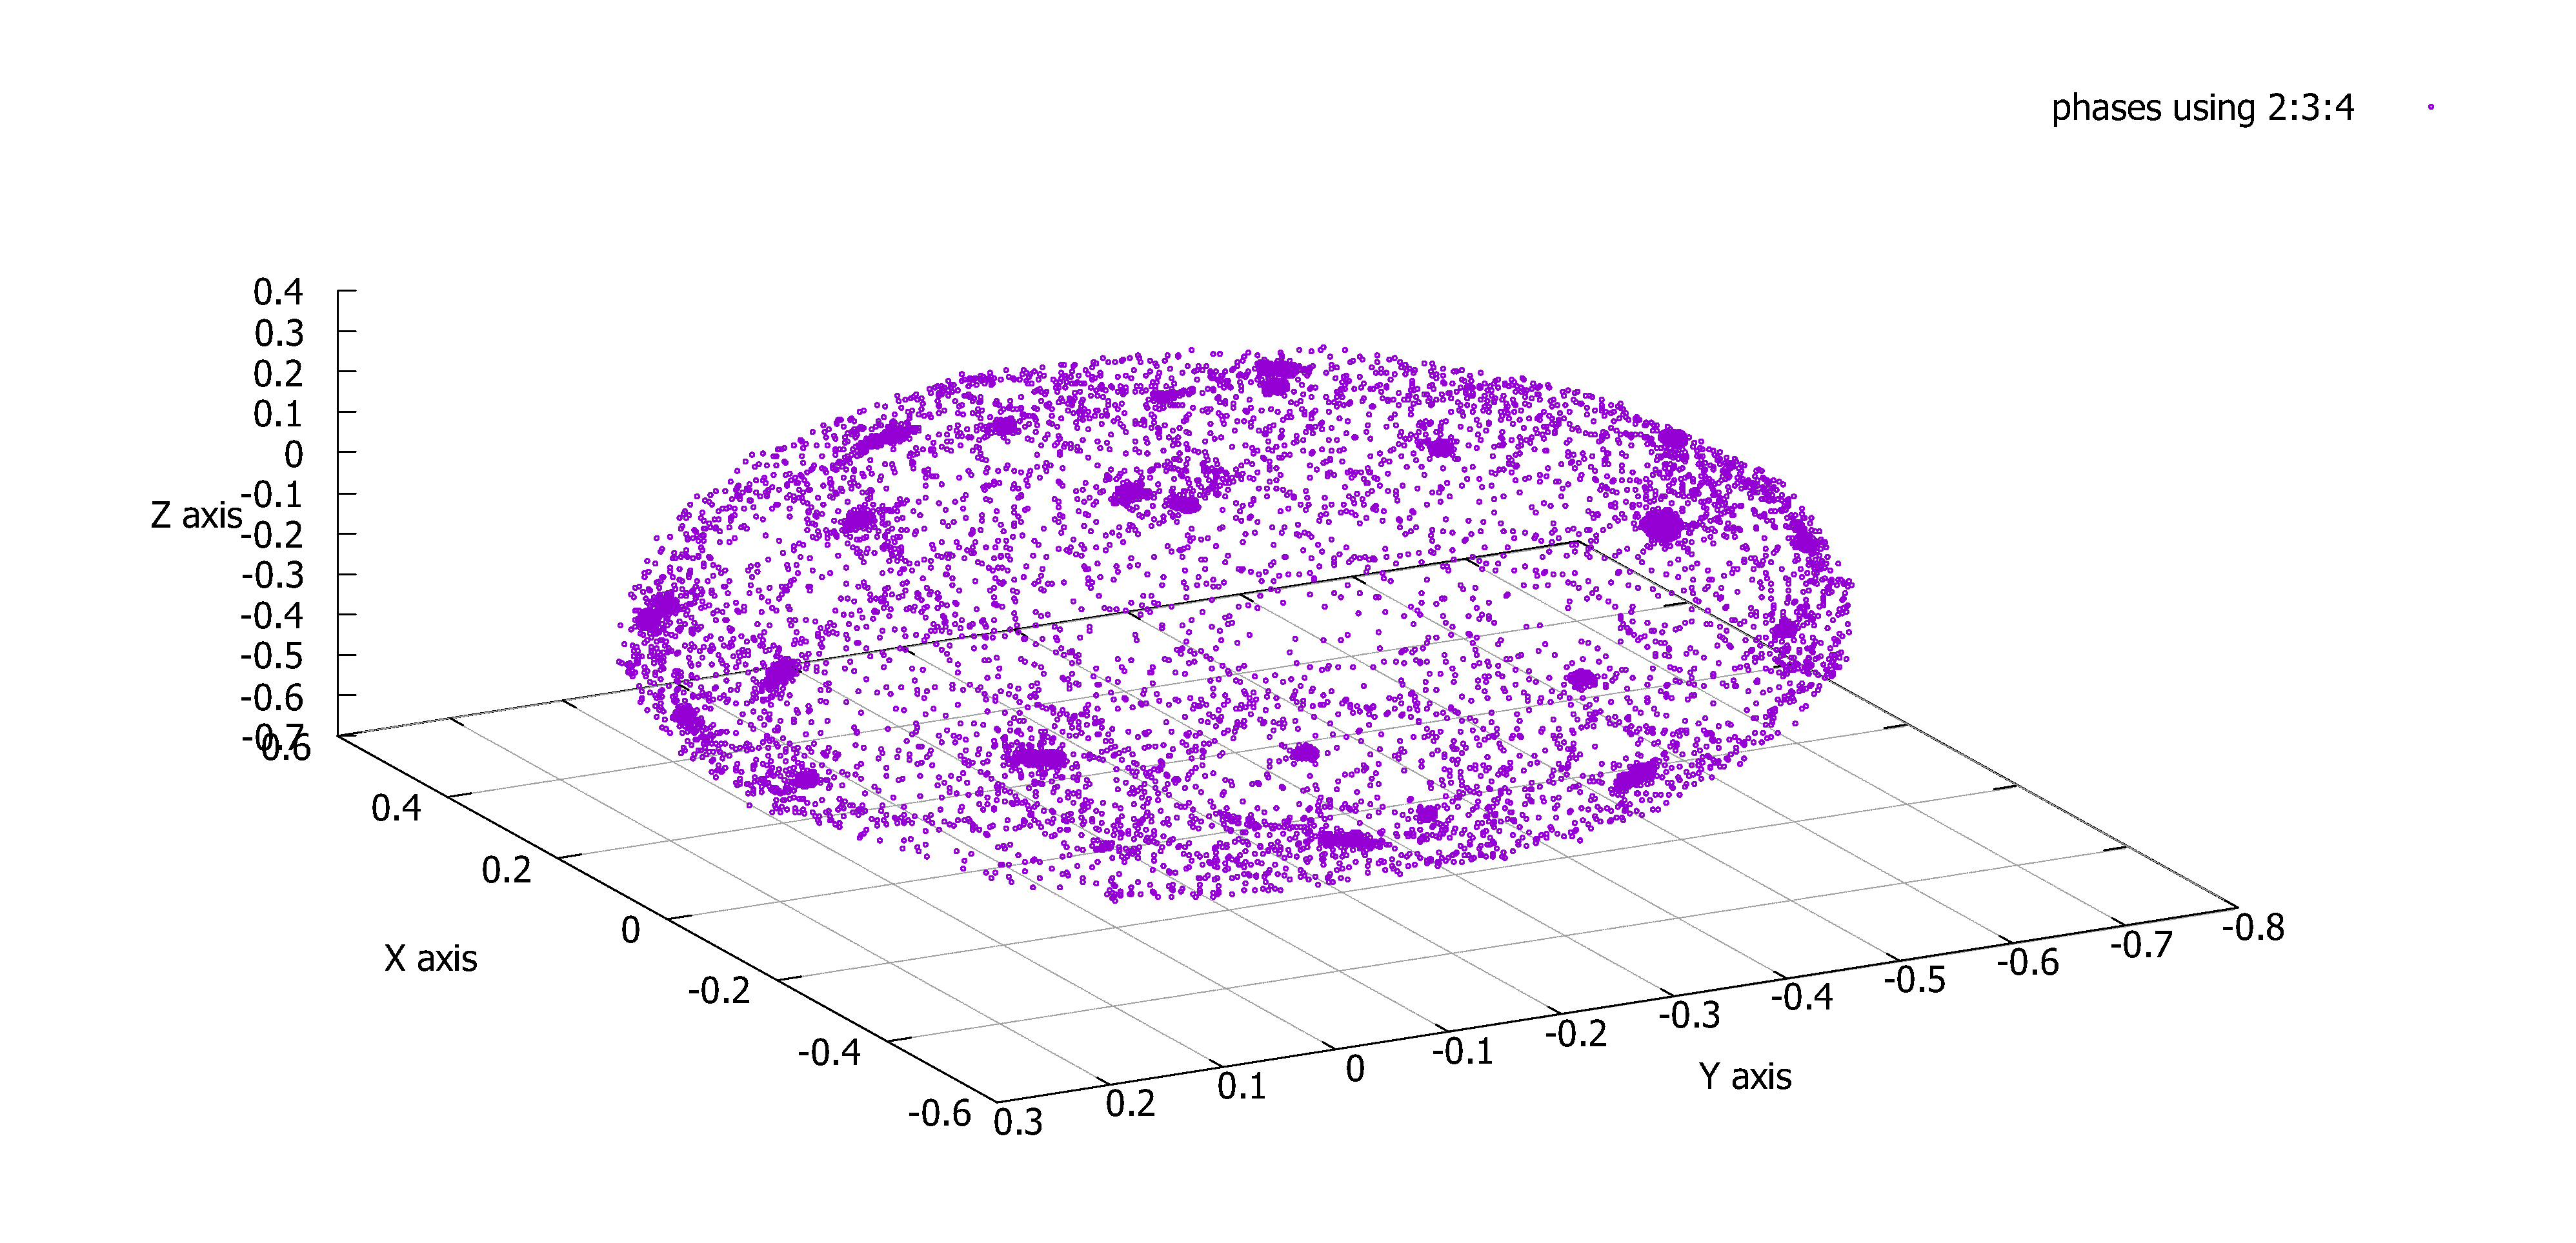
\includegraphics[width=.8\linewidth]{images/04_results/raw_sphere_calibration_phases_II_III.pdf}
  \caption{Phases II and III, combination of both.}
\end{subfigure}
\caption{Uncalibrated magnetometer components of the calibration measurement plotted in 3D-Space to form a distorted sphere.}
\label{fig:res:raw_calibration_three_phases}
\end{figure}


The final coefficients of the fit are presented in sec. \ref{sec:app:final_coefficients} in table \ref{tab:app:coeff} and the correlation matrices later in the same section. To determine the best set of parameters, the measurements are calibrated using all three sets and the residuals, i.e. the difference between calibrated vector and theoretical value, calculated. 

The residuals with mean $\mu$ and standard deviation $\sigma$ are presented in fig. \ref{fig:res:residuals}. It can be seen, that the magnetometer calibration with the lowest mean deviation from the optimal value of $503.4$\,mGs is the calibration using phases II + III. The accelerometer calibration with the lowest deviation from the optimal value of 1$g$ is using only phase II. All sets of coefficients have around the same standard deviation which are about 50 to 100 times larger than the means. This can be explained by the extremely large errors in the later stages of the measurement series. Even though it is only a small part of the dataset, an error of 100\,\% is extremely large in comparison to a mean of e.g. 0.17\,\%.
\begin{figure}[H]
    \centering
    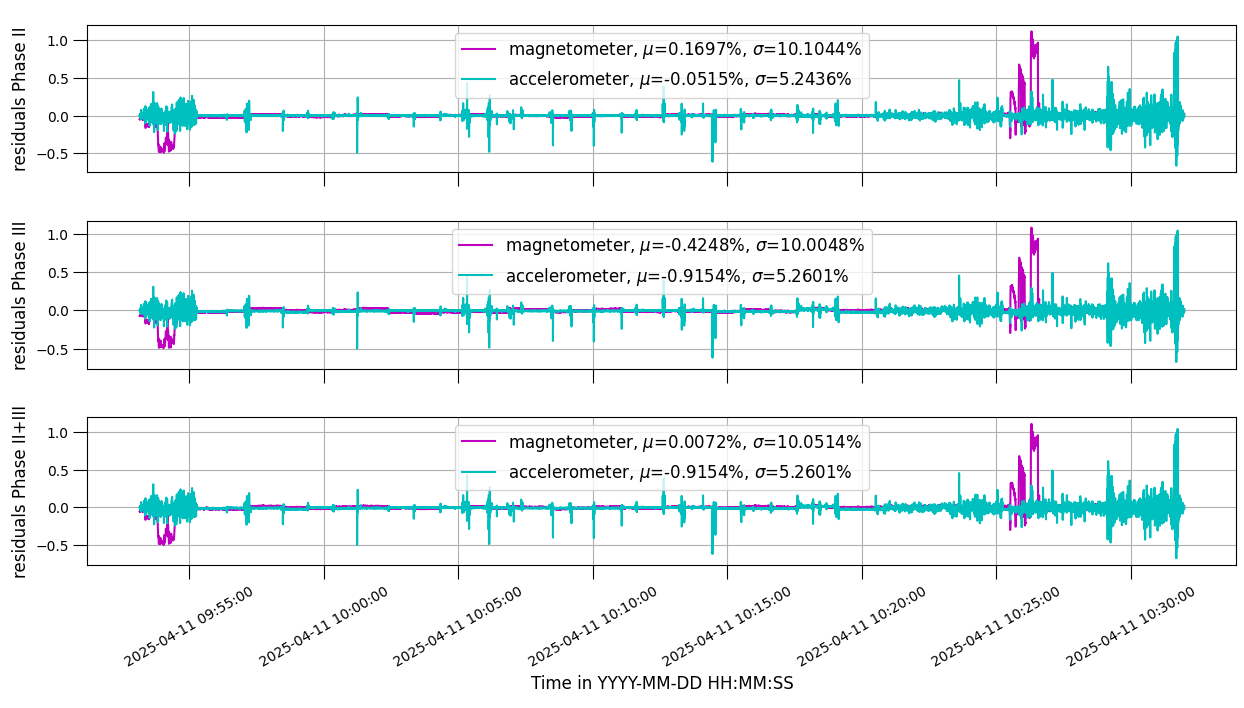
\includegraphics[width=\linewidth]{images/04_results/residuals_mag_acc_calibrations.png}
    \caption[Residuals of the calibrations.]{Residuals of the calibrations from top to bottom: Phase III, Phase II and Phases II+III.}
    \label{fig:res:residuals}
\end{figure}

The calibrated curves using only the coefficients of one set are presented at the end of sec. \ref{sec:app:final_coefficients}. The dataset calibrated using the optimal coefficients as determined above is shown in fig. \ref{fig:res:optimal_coeff_magnitude}. There it can be seen, that the magnetometer now shows a constant magnitude for the most part. Especially during the random tumble there is little deviation from the constant value aside from one time period in which the magnitude suddenly increases inexplicably.\\
The accelerometer paints a very different picture. Even with the optimal calibration coefficients, the magnitude is all but constant when continuously moving the sensor. Sensor performance cannot be improved by post-processing.  
\begin{figure}[H]
    \centering
    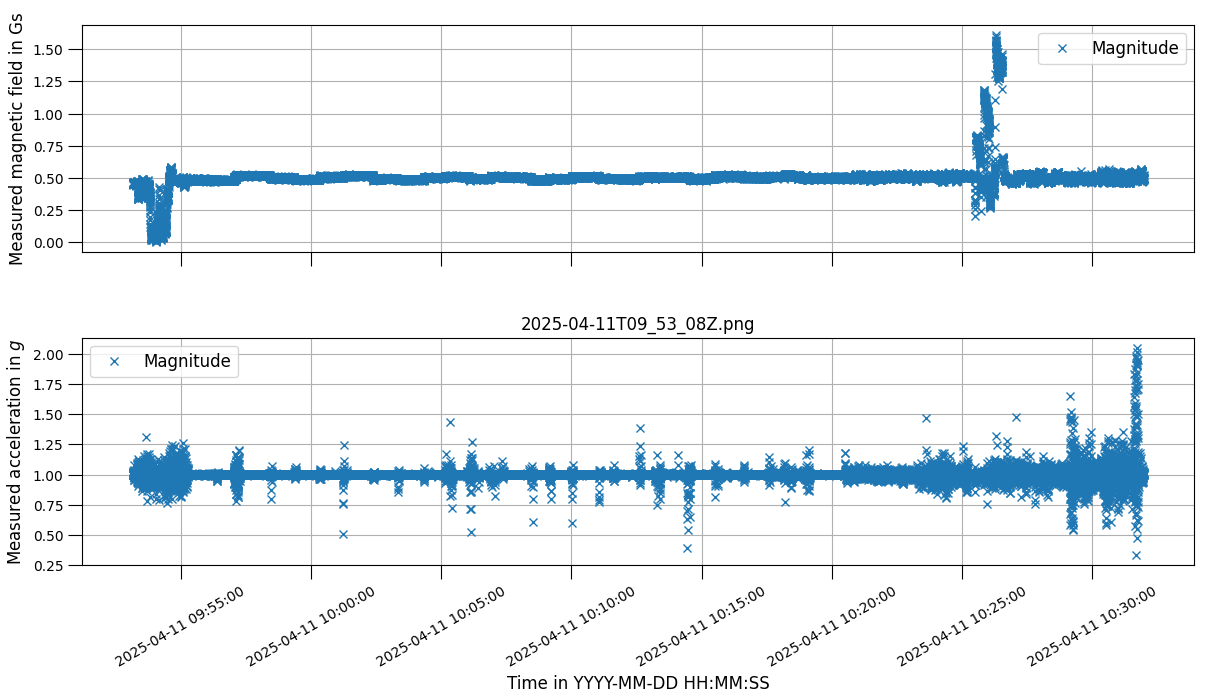
\includegraphics[width=\linewidth]{images/04_results/optimal_calibrated_11apr_magnitude.png}
    \caption{Magnitudes of magnetometer and accelerometer with optimal coefficients.}
    \label{fig:res:optimal_coeff_magnitude}
\end{figure}



\section{Attitude \label{sec:res:attitude}}
In this section we evaluate the measurements of the accelerometer to determine roll and pitch angle of the gondola.

\section{Heading \label{sec:res:heading}}
This section will present the evaluation of the magnetometer as a means of determining the gondolas direction. The attitude of the gondola has to be taken into account because...